%-----------------------------------------------------------------------------
%
%               Template for sigplanconf LaTeX Class
%
% Name:         sigplanconf-template.tex
%
% Purpose:      A template for sigplanconf.cls, which is a LaTeX 2e class
%               file for SIGPLAN conference proceedings.
%
% Guide:        Refer to "Author's Guide to the ACM SIGPLAN Class,"
%               sigplanconf-guide.pdf
%
% Author:       Paul C. Anagnostopoulos
%               Windfall Software
%               978 371-2316
%               paul@windfall.com
%
% Created:      15 February 2005
%
%-----------------------------------------------------------------------------


\documentclass{sigplanconf}

% The following \documentclass options may be useful:

% preprint      Remove this option only once the paper is in final form.
% 10pt          To set in 10-point type instead of 9-point.
% 11pt          To set in 11-point type instead of 9-point.
% authoryear    To obtain author/year citation style instead of numeric.
\usepackage[utf8]{inputenc}
\usepackage{amsmath}
\usepackage{hyperref}
\usepackage{graphicx}
\usepackage{caption}

\begin{document}

\special{papersize=8.5in,11in}
\setlength{\pdfpageheight}{\paperheight}
\setlength{\pdfpagewidth}{\paperwidth}

\conferenceinfo{CONF 'yy}{Month d--d, 20yy, City, ST, Country} 
\copyrightyear{20yy} 
\copyrightdata{978-1-nnnn-nnnn-n/yy/mm} 
\doi{nnnnnnn.nnnnnnn}

% Uncomment one of the following two, if you are not going for the 
% traditional copyright transfer agreement.

%\exclusivelicense                % ACM gets exclusive license to publish, 
                                  % you retain copyright

\permissiontopublish             % ACM gets nonexclusive license to publish
                                  % (paid open-access papers, 
                                  % short abstracts)

\titlebanner{banner above paper title}        % These are ignored unless
\preprintfooter{short description of paper}   % 'preprint' option specified.

\title{Uniforms}
\subtitle{e-Formulaire, Rapport Scientifique}

\authorinfo{Michel Gautero}
           {I3S}
           {Michel.Gautero@unice.fr}
\authorinfo{Ayoub Benathmane}
           {M2 IFI}
           {benathmane.ab@gmail.com}
\authorinfo{Genevi\`eve Cirera}
           {SI5}
           {genevieve.cirera@gmail.com}
\authorinfo{Lu\'is Felipe Polo}
           {SI5}
           {luisfelipepolo@hotmail.com}
\authorinfo{Romain Truchi}
           {M2 IFI}
           {romain.truchi.06@gmail.com}

\maketitle

\begin{abstract}
This is the text of the abstract.
\end{abstract}

\category{CR-number}{subcategory}{third-level}

% general terms are not compulsory anymore, 
% you may leave them out
\terms
term1, term2

\keywords
Uniforms, form

%-----------------------Section introduction
\section{Introduction}
De nos jours, deux types de formulaire existent. Les formulaires papiers, distribués puis collectés physiquement et les formulaires électroniques, qui peuvent être envoyés par e-mail, les destinataires répondent alors par l’intermédiaire d’une page web leur affichant les questions et les champs de réponses possibles.\\
L’idée générale de ce projet est de proposer une manière de concevoir les formulaires, les partager et les gérer sans avoir recours à une application externe à l’université de Nice Sophia-Antipolis car de nombreuses applications de création de formulaire existantes collectent et conservent les données sur leurs serveurs. Il faut également que notre application puisse proposer les deux types de transmission, physique, grâce à une fonctionnalité d’impression des formulaires, et électronique.\\
D’autres points sont essentiels à ce projet comme le besoin de proposer une interface instinctive à l’utilisateur, qu’il puisse comprendre facilement le fonctionnement de l’application et qu’il ne perde pas de temps, que l’application soit bénéfique tout autant dans le temps que par les possibilités de création et de gestion par rapport à ses moyens actuels. \\
De plus, l’application devra être compatible avec les technologies de l’université car elle y sera hébergées.\\

Nous verrons tout d'abord les scénarios justifiants du besoin de cette application, puis la description de notre contribution, les tests réalisés, le positionnement de notre application par rapport à l'état de l'art pour enfin conclure.


%------------------Section scénario
\section{Un exemple}
Notre problème se décompose en plusieurs scénarios distincts, la création/modification de formulaire, la consultation des réponses, la réalisation des réponses à un formulaire non anonyme et anonyme et le remplissage de formulaire papier. Nous pouvons voir un résumé de tous ces scénarios figure~\ref{scenarios} avec leurs descriptifs figure~\ref{listScenarios}.

\noindent\begin{minipage}{\linewidth}% to keep image and caption on one page
\makebox[\linewidth]{%        to center the image
  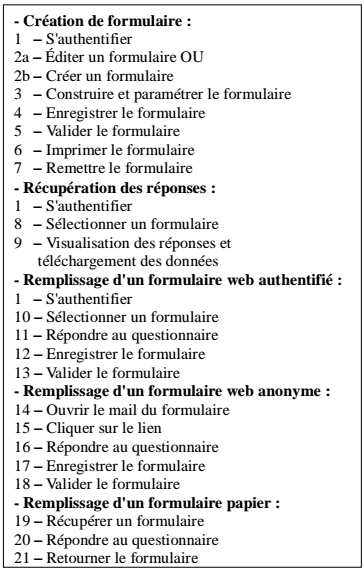
\includegraphics [width=70mm]{images/listScenarios.png}}
\captionof{figure}{Descriptif des scénarios}\label{listScenarios}
\end{minipage}

\subsection{S'authentifier}
L’utilisateur doit tout d’abord s'identifier avec le CAS\footnote{Central Authentification Service} ou localement. Ensuite, il aura accès aux formulaires qui lui sont destinés et aux fonctionnalités de création.

\subsection{Créer un formulaire et le soumettre}
Une fois authentifié, l'utilisateur peut cliquer sur “Créer un formulaire”, une interface lui sera proposée afin qu’il puisse placer les éléments par drag’n’drop là où il le souhaite. Label pour écrire une question, des boutons radios ou checkbox pour une question à choix multiple…\\
L’utilisateur peut également former des groupes d’éléments afin de les assigner à une personne précise. C’est-à-dire que la personne assignée à un groupe d’éléments sera la seule personne autorisée à remplir ces champs là (cette fonctionnalité sera très utile si le formulaire est une demande d’autorisation que que la même personne doit donner son accord pour toutes les demandes).\\
L’utilisateur peut ensuite définir les paramètres pour que le formulaire soit imprimable et/ou anonyme. Si ce dernier est anonyme alors il ne sera pas nécessaire de se connecter pour répondre à ce formulaire et les personnes pouvant répondre à ce formulaire sont celles disposant du lien.\\
Si le formulaire est imprimable alors les éléments seront arrangés de telle manière à ce qu’ils puissent être sur une page A4.\\
De plus, l’utilisateur peut définir un nombre de réponse accepté par personne pour un même formulaire, de 1 à l’infini.\\
Après ces paramétrages, l’utilisateur peut soit enregistrer, soit publier le formulaire. Dans ce dernier cas, le formulaire sera pourra être rempli par ses destinataires et il ne pourra plus être modifié.\\

\noindent\begin{minipage}{\linewidth}% to keep image and caption on one page
\makebox[\linewidth]{%        to center the image
  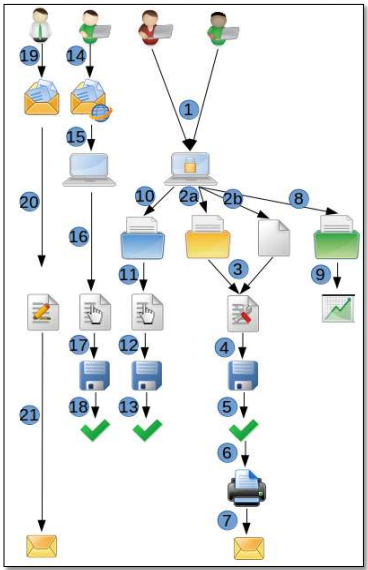
\includegraphics [width=70mm]{images/scenarios.png}}
\captionof{figure}{Scénarios}\label{scenarios}
\end{minipage}

\subsection{Créer un formulaire avec des groupes}

\subsection{Modifier un formulaire}
Les formulaires enregistrés peuvent être modifiés. Parmi toute la liste des formulaires qu’il a créés, l’utilisateur peut modifier ceux qui ne sont pas publiés. Dans ce cas, la page de création de formulaire lui est présentée préremplie par les informations enregistrées du formulaire en cours de construction. 

\subsection{Consulter les réponses}
Le créateur peut consulter les réponses des formulaires qu’il a créés. Pour cela, il doit s’identifier sur la plate-forme, puis aller sur la page de consultation des réponses du formulaire souhaité. Les réponses s’affiche aux fur et à mesure que les destinataires répondent au formulaire.\\
Les réponses peuvent être consultées directement sur l’application ou bien être téléchargées en CSV et/ou SQL.\\
%ne faudrait-il pas développer ? Pourquoi deux formats ? Comment et par qui peuvent être utilisés ces formats ? Quelles connaissances/logiciels nécessitent-ils ? Quels avantages et inconvénients ?

\subsection{Répondre à un formulaire}
Pour les formulaires non anonymes, les destinataires doivent tout d’abord s’identifier pour pouvoir répondre à un formulaire. Ils accèdent alors à l’ensemble des formulaires dont ils sont destinataires, ils peuvent alors y répondre. \\
Une fois répondu, ils ont le choix entre enregistrer la réponse ou l'envoyer. “Enregistrer” permet de modifier la réponse plus tard, “Envoyer” envoie la réponse au créateur du formulaire, elle ne sera plus modifiable.\\
Pour les formulaires anonymes, aucune identification n’est obligatoire, les personnes possédant le lien du formulaire peuvent y répondre, en revanche enregistrer une réponse pour la modifier plus tard est impossible car anonyme, le formulaire doit être rempli en une seule fois.

\subsection{Soumission de formulaire papier}
Le créateur dispose d’une fonctionnalité d’impression du formulaire, il peut alors distribuer les formulaires en main propre et collecter les réponses physiquement. \\


%--------------------------Section technologie
%\section{Contribution}
\section{Choix des technologies}
Le choix des technologies s’est fait très rapidement en début de projet, nous avons décidé des langages, librairies, frameworks et outils de gestion de projet.
\subsection{Langages}
\subsubsection{Coté serveur}
Pour réaliser un site dynamique comme le notre, il est nécessaire d'utiliser un langage serveur.\\
Plusieurs langages sont disponibles, ASP\footnote{Active Server Pages} .NET, Ruby on Rails, Django, JEE\footnote{Java Enterprise Edition},... Tous ont leurs avantages et inconvénients.\\
ASP .NET exploite le framework .NET, est très proche du développement en C\# et est propriétaire, Django au contraire est un framework Python open-source, JEE pour les développeurs Java...\\
Au niveau des services des frameworks, Django et Ruby on Rails sont en tête, cependant, les services proposés ne nous sont pas forcément nécessaires. Pour contruire une application web ``simple'' et n'ayant pas tous les mêmes compétences, PHP\footnote{Hypertext Preprocessor} nous a paru la meilleure option car, pour ceux d'entre nous ne connaissant aucun de ces langages, le temps d'apprentissage est relativement court ce qui permettrait un avancement plus rapide. De plus, nous ne perdons pas la possibilité d'exploiter l'orienté objet.\\

Pour la base de données, plusieurs SGBD\footnote{Système de Gestion de Base de Données} sont possibles, Oracle, PostgreSQL, MySQL, MongoDB...\\
Oracle est propriétaire, MongoDB est un SBGD NoSQL\footnote{Not only SQL}, PostgreSQL et MySQL quant à eux sont libre et relationnel.\\
Pour notre application, nous avions besoin d'un SGBDR\footnote{Système de Gestion de Base de Données Relationnelles}, MySQL et PostgreSQL paraissaient donc de bonnes options.\\

Nous avions également une contrainte de déploiement, l'application devait pouvoir être hébergée à l'UNS\footnote{Université de Nice Sophia-Antipolis}, PHP\cite{urlPHP} et MySQL\cite{urlMySQL} était donc les seuls choix possibles.\\
Les versions utilisées sont les suivantes : 
\begin{description}
\item [PHP] : 5.4.* utilisé en orienté objet
\item [MySQL] : 5.5.*
\end{description}

\subsubsection{Coté client}
Plusieurs langages sont nécessaires coté client, un langage de balisage (HTML\footnote{Hypertext Markup Language}, XML\footnote{eXtended Markup Language}, Latex,...), un langage de script (JavaScript, ActionScript, JScript, VBScript\footnote{Microsoft Visual Basic Scripting Edition},...) et des feuilles de style (CSS\footnote{Cascading Style Sheets}).
\begin{itemize}
\item Langage de balisage\\
Parmis tous les langages étudiés, HTML nous a paru le plus adapté car multiplateforme, tous les navigateurs le reconnaissent et est facile à mettre en place, peu de connaissances sont nécessaires.
\item Langage de script\\
JScript est une adaptation de JavaScript par Microsoft, VBScript a été développé par Microsoft et est un sous-ensemble de Visual Basic, il est donc propre à Microsoft.\\
JavaScript étant le langage le plus utilisé et étant reconnu par tous les navigateurs, nous avons décidé de l'utiliser.
\end{itemize}

De plus, la facilité et simplicité d'utilisation, la rapidité d'apprentissage des langages et la contrainte de déploiement nous ont mené vers le choix de HTML, CSS et JavaScript.\\
Les versions utilisées sont les suivantes :
\begin{description}
\item [HTML5]
\item [CSS3]
\end{description}

Cependant, tout développer depuis zéro, nous paraissait trop long et fastidieux, de plus, javaScript peut avoir des résultats différents suivant les navigateurs, c'est pourquoi nous avons décidé d'utiliser des librairies et frameworks.

\subsection{Librairie/Framework}
Nous avons choisi JQuery\cite{urljQuery}, une librairie JavaScript libre, pour sa simplicité et efficacité afin de faciliter l'écriture de scripts coté client.\\
Certaines fonctionnalités comme le drag’n’drop est plus facile à implémenter depuis cette librairie qu’en JavaScript pur. JQuery propose de nombreuses fonctionnalités telles que le parcours et modification du DOM\footnote{Document Object Model}, gestion des événements, création d'effets visuels et d'animations,...\\
JQuery est une librairie relativement complète mais n'est pas un framework, ce qui veut dire que le développement de l'application ne sera pas ``enfermé'' et nous garderons une certaine liberté de développement.\\

En ce qui concerne le design, il nous paraissait difficil de créer toutes les feuilles de style, en définissant les couleurs, dispositions, formes,...de chaque élément. C'est pourquoi, nous avons choisi d’utiliser Bootstrap\cite{urlBootstrap}.\\
À la différence de ses concurrents (par exemple Foundation from Zurb) Bootstrap est plus simple d’utilisation, son apprentissage est rapide et il propose des styles prédéfinis sans besoin de configuration préalable.\\
Bootstrap nous a ainsi permit de réaliser une application responsive avec un style prédéfini Bootstrap sans trop de difficulté.\\
Les versions utilisées sont les suivantes :
\begin{description}
\item [JQuery] : 2.1.1
\item [Bootstrap] : 3.3.1
\end{description}

Il nous a fallu investir du temps d'apprentissage pour ces deux technologies, cependant, ce temps était nécessaire afin d'être plus efficace pour le reste du développement.

\subsection{Gestion de projet}
Pour la gestion de notre projet, deux outils principaux ont été utilisés. Un outil de gestion de version git avec un dépôt privé sous Github et un gestionnaire de tâches sur la plateforme JIRA.\\
Le gestionnaire de version nous permet de partager du code et de travailler collaborativement.\\
Le gestionnaire de tâches est un système de tickets, l’équipe en définit tout un ensemble et chaque membre réalise les tâches qui lui sont attribuées. Chaque membre place le ticket en zone “Progress” puis “Done” une fois terminée ainsi nous avons pu suivre l’avancée de chaque membre et éviter les conflits de merge avec le gestionnaire de version.\\
Les tâches ont été définies de telles manière à suivre la méthode agile décrite dans le DoW\footnote{Description Of Work} et pouvoir progresser en lot.

%------------------------Section management
\section{Management}
\subsection{Planning prévisionnel}
\subsection{Planning réalisé}
%là, il faut tout développer, expliquer les difficultés de rdv, l'arrivée d'un nouveau membre, la découverte du problème des multi-groupes, les modifications qui en ont découlées. Il faut montrer votre adaptabilité aux événements
%------------------------Section architecture
\section{Architecture}
L'architecture figure~\ref{fonctionnementAppli} mise en place est assez simple. A gauche, les pages de notre application développées principalement avec les standards du web HTML, CSS et JavaScript avec l’utilisation du framework Bootstrap,  de l'autre un serveur d'application Apache pour interprété le code PHP qui permet de requêter ma base de données MySQL et fournir du résultat sous forme des pages HTML, Les échanges entre ces deux plateformes ceux font via le protocole HTTP.

\noindent\begin{minipage}{\linewidth}% to keep image and caption on one page
\makebox[\linewidth]{%        to center the image
  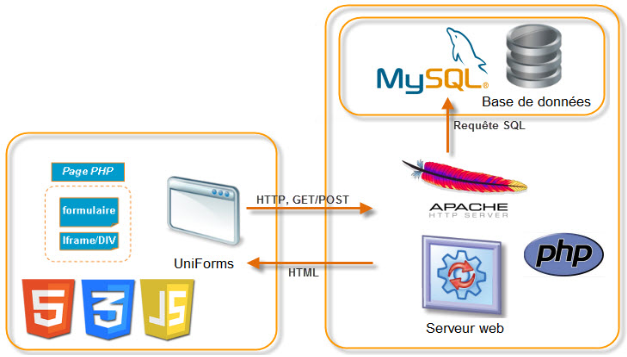
\includegraphics [width=90mm]{images/architecture.png}}
\captionof{figure}{Fonctionnement de l'application}\label{fonctionnementAppli}
\end{minipage}

\subsection{Base de données}
%il faut développer l'aspect bd, l'aspect objet et peut-être en profiter pour montrer ce qu'il faut faire pour ajouter un composant -> cela montrera comment étendre votre projet
\subsection{Classes PHP}


\section{Connexion et compte}
\subsection{CAS}
\subsection{Session}
%---------------------------------Section fonctionnalité développées----------------
\section{Les fonctionnalités développées}
\subsection{Création/Modification de formulaire}
\subsubsection{Éléments choisis (lesquels/pourquoi)}
Douze éléments sont proposés. Ils ont été choisis de manière stratégique afin de proposer un ensemble assez divers, que l’utilisateur puisse exprimer ce qu’il souhaite tout en prenant en compte les contraintes de temps qui nous étaient imposées pour la réalisation du projet.\\
Ainsi l’utilisateur peut mettre des questions (grâce aux labels), mettre des champs de réponses de questions à choix multiples (bouton radio et cases à cocher), mettre des champs simples (input text, paragraphe),... Mais aussi, il peut dessiner des zones grâce au carré et au cercle ainsi qu’ajouter par exemple un logo grâce à l’insertion d’images.

\subsubsection{Destinataires}
Pour la sélection de destinataires, un champs d’entrée est proposé. Dans ce champs à chaque entrée de caractère, des propositions de destinataires sont affichées.\\
Ce choix pour la sélection de destinataires a été fait pour palier au grand nombre de destinataires qui seront disponibles. En effet, ce nombre peut atteindre deux ou trois milles, l’affichage de tous les destinataires sur une page n’étaient donc pas adapté.\\
D’autre part, la sélection de destinataire se fait par identifiant CAS, c’est-à- dire que le créateur doit connaître les identifiants des personnes à qui il souhaite envoyer le formulaire. Ce choix est dû au fait que l’on ne possédait pas assez d’informations pour lier les noms, prénoms, promotion aux identifiants de connexion CAS.

\subsubsection{Paramètres (lesquels et pourquoi avoir choisi ces paramètres)}
Trois paramètres nous ont paru indispensables et suffisants. 
\begin{itemize}
\item “Imprimable” car dans les objectifs du DoW mais pas forcément obligatoire pour chaque formulaire.
\item “Anonyme” pour pouvoir offrir la possibilité de faire un sondage comme les concurrents sans connaître l’identité des personnes et donc soumettre un formulaire à des personnes externes à l’université.
\item “Nombre de réponses max” afin de ne pas avoir à recréer un même formulaire pour obtenir plusieurs réponses d’une même personne.
\end{itemize}
Ces paramètres sont ensuite traités en PHP grâce à une requête POST\footnote{HyperText Transfer Protocol} envoyée à l’enregistre ou à la validation du formulaire.

\subsubsection{Glisser-déposer}
Un glisser-déposer aussi appelé drag'n'drop a été implémenté en JQuery afin de donner la possibilité de créer le formulaire le plus proche possible de la réalité. Le champs disponible pour la position des éléments est de la taille d’une page A4, une fois rempli la page s’agrandit d’une page en hauteur.\\
L'ensemble des éléments positionnés est au fur et à mesure enregistré grâce à des objets JavaScript, on peut ainsi récupérer les paramètres que l'utilisateur renseigne.\\
Pour la formation de groupes, c’est le même principe, sauf que les informations des groupes ne sont récupérées qu’à la fin, au moment de l’enregistrement (ou validation) car aucun paramètre n’est à renseigner.\\
Lors de l’enregistrement (ou validation), deux variables sont envoyées en requêtes POST pour le détails des éléments et groupes créés par l’utilisateur.

\subsection{Répondre à un formulaire}

\subsection{Consulter les réponses aux formulaires}
\subsubsection{En ligne}
\subsubsection{Télécharger les résultats}

%---------------------------Section Validation
\section{Validation}
Lorsque l'application est réalisé, il convient que notre encadrant s'assure qu'il répond aux objectifs cités dans le Description Of Work, pour cela nous avons programmé des réunions après la fin de chaque lot dans le but d’assurer le bon avancement du projet en fonction des objectifs attendues.

\subsection{Outils de tests utilisés}
Afin de réaliser les tests nous avons utiliser deux outils, SimpleTest pour les tests des classes PHP et Sélénium IDE pour les tests de scénarios.\\
Malgré que PHPUnit soit un standard des framework de tests PHP, nous avons choisi SimpleTest car il possède une interface web pour l’exécution des tests. De plus, l’équipe travaillant sur deux systèmes d’exploitation différents, SimpleTest fonctionnait sur les deux à la différence de PHPUnit.\\
Selenium est un plugin fonctionnant sur de nombreux navigateurs (Firefox, Chrome, Opéra,...) permet de tester les scénarios.

\subsection{Tests classes PHP}
Afin de vérifier le bon fonctionnement des méthodes de nos classes PHP, nous les avons testé en utilisant SimpleTest.

\subsection{Tests scénarios}
Sélénium IDE pour les tests d’interface

\subsection{Tests utilisateurs}
Nous avons essayé de faire appel à des personnes de l’université qui n’ont jamais entendu parlé de ce projet, leurs réactions ne seront donc pas influencées et nous pourront noter les facilités et/ou difficultés rencontrées et ainsi améliorer l’utilisabilité. Malheureusement nous n’avons pas pu le faire pour la simple raison que les créneaux consacrés pour le projet de fin d'étude en temps complet coïncident avec les vacances universitaires, c’est pourquoi il a été difficile pour nous et pour notre encadrant pour trouver des personnes disponibles.

%------------------------------Section Positionnement
\section{Positionnement}
Ici, nous allons positionner notre application par rapport à l’état de l’art. Tout d’abord nous allons la confronter aux logiciels classiques puis aux e-formulaires existants du web.
\subsection{Face aux logiciels classiques}
Dans l’état de l’art nous avions étudié trois logiciels,  Microsoft Office (Word et Excel), Adobe (PDF LiveCycle Designer) et Latex.\\
Le défaut commun à ces trois logiciels étaient qu’ils demandaient tous un minimum de connaissances informatiques.\\
Notre application se démarque de ces dernières car permet de réaliser la même chose que ces logiciels mais sans avoir besoin nécessairement de connaissances informatiques. Uniforms propose une interface graphique pour tout, de la création des formulaires à la consultation des réponses en passant pas la réalisation des réponses et n’a pas besoin d’écrire de code.
Un autre défaut majeur est que les logiciels Microsoft Office et Adobe sont payants et accessibles par le système d’exploitation Windows uniquement, ce qui restreint le nombre d’utilisateur potentiel et dans l’autre sens également, les personnes souhaitant créer des formulaires n’ont pas tous accès à ces outils. En revanche, notre application web est accessible depuis n’importe quel système d’exploitation et est totalement gratuite.
De plus, certain outil tel que Word ne propose pas une variété d’éléments suffisants, seulement des champs de texte simple, pas de spécification pour un champ de date, d’heure ou de numéro de téléphone…\\
Uniforms a été développée de manière à proposer à l’utilisateur un outil accessible à tous sans les inconvénients cités précédemment.

\subsection{Face aux e-formulaire}
De nombreux e-Formulaires sur le web proposent des interfaces graphiques pour réaliser des formulaires. Tous proposent des interfaces plus ou moins instinctives, l’utilisateur n’a pas besoin d’écrire de code. \\
Ici, nous allons comparer ces applications à Uniforms sous divers points de vue.
\subsubsection{Utilisabilité}
Les applications existantes n’obligent pas forcément l’utilisateur à se connecter, c’est pourquoi, il doit créer le formulaire ne une fois, sans pause ni coupure de connexion. Pour un meilleur confort de l’utilisateur, nous avons pensé à implémenter la fonctionnalité d’enregistrement pour modification et validation plus tard tout autant dans la création de formulaires comme dans les réponses faites par les destinataires.\\
Pour une meilleure efficience, nous avons également pensé à proposer un système de placement des éléments sur la page là où l’utilisateur le souhaite, c’est-à-dire que le créateur dispose d’un drag’n’drop là où il le souhaite sur la page et non les disposer les uns sous les autres de manière verticale comme le propose WebQuest par exemple. Également, l’utilisateur n’est pas obligé de placer des groupes de une question et un champs de réponse comme bons nombres des applications existantes. Cela laisse la liberté de création à l’utilisateur.\\
Au niveau de l’efficacité, elle est comparable aux applications existantes car le système est similaire, drag’n’drop d’éléments sur la page et renseignement des propriétés des éléments (requit, taille,...).\\
Les applications existantes proposent une version mobile, notre application est réalisée avec Bootstrap, donc responsive, mais la page de création devant être imprimable a donc une taille de page A4, il n’est donc pas possible de créer un formulaire sur un mobile, mais la consultation, téléchargement des résultats est possible. Pour ce point, les applications existantes surpassent notre application.\\
Pour ce qui est de l’interface, elle est simple, intuitive et un manuel d’utilisation a été rédigé afin d’en faciliter l’utilisation tout comme pour les application existantes.
\subsubsection{Éléments proposés}
Les éléments proposés dans notre application sont au nombre de douze (label, nombre, champs texte, paragraphe, boutons radios, cases à cocher, date, heure, numéro de téléphone, image, carré et cercle). D’autres application telles que Oxiform ou Typeform en propose plus en y ajoutant le champs d’url, d’email, de liste déroulante...à ceux que nous proposons.\\ Cependant, notre application n’est pas totalement mal placé car certaines applications proposent moins d’éléments, WebQuest n’en propose que huit.
\subsubsection{Anonymat}
La question de l’anonymat à la réponse d’un formulaire se pose très souvent. Les destinataires doivent-ils être identifié ou non ? L’entrée de leurs identifiants (nom, prénom, numéro,...) est-elle suffisante pour que le créateur soit sur que la réponse a été effectuée par un certain destinataire.\\
Sur le web, la majorité des applications de création de formulaire ne propose pas d’identification, n’importe quelle personne étant en possession du lien du formulaire peut y répondre. Par exemple, Oxiform ou Typeform. \\
Nous avons voulu y rémédier, notre application propose de créer des formulaires anonymes ou non, ce qui permet de faire des sondages sans se soucier de qui répond au formulaire tout comme les applications déjà existantes, mais aussi de créer des formulaires nominatifs, ajouter des destinataires précis grâce au système d’identification CAS intégré.
\subsubsection{Confidentialité}
Toutes les applications du web stockent les données dans le Cloud, ce qui veut dire que les applications existantes disposent d’autant de données que de champs de formulaire remplis par les destinataires. Pour ce point là, uniforms a pour principal but de se mettre au service de l’université, il y est hébergé, les données ne sont donc pas partagées avec un tiers.
\subsubsection{Design}
Des applications telles que Oxiform ou Typeform proposent des thèmes. Notre application n’a pas pour cet objectif, mais plutôt celui de rendre le formulaire imprimable, le thème “noir sur blanc” est donc tout à fait justifié.
\subsubsection{Exportation}
Diverses méthodes d’exportation sont disponibles avec les applications existantes, xml, csv, xls pour Formpro, intégration à une page web existante pour Oxiform. Notre application ne propose que l’exportation en csv, sql et la consultation des résultats en ligne. Les résultats sont exportables par moins de moyens et aucune option de statistiques sur résultats n’est possible à la différence de Formpro.
\subsubsection{Gratuité}
Notre application est totalement gratuite, toutes les applications existantes auxquelles nous avons comparé uniforms précédemment sont soit limités en nombre de formulaire ou dans le temps (sauf Google Form).

\subsection{Synthèse}
Nous avons précédemment comparé notre application à celles existantes sous divers aspects. En général, nous avons vu que notre application se démarquait pour certains aspects comme la confidentialité, l’anonymat ou même la gratuité.\\
En revanche, sous d’autres aspects, elle est plus faible, par exemple le nombre d’éléments disponibles qui, en moyenne, est plus élevé. L’exportation de données ne se fait que sous deux formes alors que d’autres applications proposent beaucoup plus. Cependant, l’objectif de notre application n’est pas l’exportation, mais plutôt de pouvoir gérer les résultats en dehors de l’application, l’objectif est donc atteint. \\
Au niveau du design, notre application a pour but d’être imprimable, il est donc normal de ne pas proposer de thèmes comme les applications existantes.\\
En ce qui concerne l’utilisabilité, elle se positionne au même niveau que les applications existantes, ergonome et instinctive malgré le fait qu’elle ne propose pas de version mobile, elle propose néanmoins des possibilités de modification (formulaire ou réponse).

%--------------------------Section Conclusion
\section{Conclusion}
\subsection{Résultats obtenus}
Au début du projet, cinq critères de succès ont été définis et six objectifs ont été fixés.\\ 
Nous allons ici voir ce qui a été réalisé. 
\subsubsection{Objectifs}
\begin{itemize}
\item Uniformiser la représentation d'un formulaire\\
L’application propose bien une représentation imprimable proche de celle réalisée par l’utilisateur.
\item Présenter une interface utilisateur ergonomique\\
C’est un des points les plus importants pour notre application, la facilité d’utilisation pour un non informaticien, une interface intuitive. Notre tuteur qui a également le rôle de client nous a conseillé pour le développement de l’interface et a confirmé son utilisabilité. Ce point est donc validé et valide également un critère de succès.
\item Garantir la confidentialité des données\\
L’authentification CAS permet de nominer les créateurs et les destinataires. De plus, l’application étant hébergée à l’université, cela permet de ne pas avoir à partager les données avec un tier. Ce point valide également un critère de succès.
\item Permettre la gestion de collections de formulaires\\
Uniforms permet la gestion des formulaires créés et des formulaires reçus, avec les quatre opérations CRUD\footnote{Create Read Update Delete}, création, lecture, mise à jour et suppression.
\item Donner la possibilité de pré-remplir des champs\\
Ce point là a été abandonné en cours de projet, car la fonctionnalité de création de formulaire dit “Collaboratif” a dû être revu et son temps de développement a augmenté pour prendre en compte certains éléments importants (ordre de remplissage, nombre de réponses autorisée,...). Avec accord du client, nous avons décidé de développer le formulaire “collaboratif” et d’abandonner le pré-remplissage.
\item Livrer une documentation\\
Deux documentations ont été réalisées. Une documentation technique à l’aide de PHPdoc pour les éventuels futurs développeurs qui souhaiteraient reprendre le projet et un manuel utilisateur afin d’expliquer en détail le fonctionnement de l’application aux utilisateurs.\\
Cette documentation valide également un critère de succès.
\end{itemize}

Les autres critères de succès, génération de formulaire papier exploitable et création d’un package sont également validés car lors de la création d’un formulaire, l’utilisateur peut imprimer son formulaire grâce à la combinaison de touche Ctrl + P. Il peut ainsi vérifier sa mise en page finale. Pour le package d’installation…
\subsubsection{Synthèse}
Pour conclure sur les résultats obtenus, nous pouvons dire que tous les critères de succès ont été atteints. Hormis l’objectif du pré-remplissage des champs qui est compensé par le formulaire “collaboratif”, tous les objectifs ont également été atteints.

\subsection{Perspectives}
À la vue de nos résultats et de l’état de l’art, on pourrait imaginer diverses améliorations.\\
Premièrement, au niveau des utilisateurs. Actuellement, les utilisateurs autorisés sont ceux pouvant s’identifier avec CAS. Il pourrait être intéressant d’ouvrir le champs des utilisateurs à des personnes externes à l’université. Par exemple, si l’on souhaite recueillir l'opinion de personne ayant assistée un événement de l’université. Un compte temporaire serait créé pour qu’ils répondent au formulaire. À la différence d’un formulaire anonyme, les personnes qui répondront seront définies.\\
Deuxièmement, la liste des éléments disponibles est limitées, proposer plus d’éléments comme un champs d’url, d'adresse mail, liste déroulante... \\
Troisièmement, les champs de réponses sont vides lorsqu’ils sont proposés au destinataire, il serait pertinent de développer la fonctionnalité d’auto-remplissage par bases de données externes. Par exemple, si le créateur possède en local une base de données concernant les promotions de chaque élève, qu’il puisse, par l’intermédiaire d’un script qu’il écrira, remplir les champs de promotion de élève du formulaire soumis.




\appendix
%\section{Appendix Title}

%This is the text of the appendix, if you need one.

%\acks

%Acknowledgments, if needed.

% We recommend abbrvnat bibliography style.

\bibliographystyle{abbrvnat}

% The bibliography should be embedded for final submission.

\begin{thebibliography}{}
\softraggedright
\bibitem{urlPHP} Site web PHP : \url{http://php.net/}
\bibitem{urlMySQL} Site web MySQL : \url{http://www.mysql.fr/}
\bibitem{urljQuery} Site web jQuery : \url{http://jquery.com/}
\bibitem{urlBootstrap} Site web Bootstrap : \url{http://getbootstrap.com/}

\end{thebibliography}


\end{document}

%                       Revision History
%                       -------- -------
%  Date         Person  Ver.    Change
%  ----         ------  ----    ------

%  2013.06.29   TU      0.1--4  comments on permission/copyright notices

